\documentclass[12pt]{article}

\usepackage{float}
\usepackage[pdftex]{graphicx} 
\graphicspath{{../img/}}
\DeclareGraphicsExtensions{.pdf,.jpeg,.png,.jpg} 

\usepackage{listings}
\lstset{language=Python, keywordstyle=\color{blue}, stringstyle=\color{olive}, breaklines=true, showstringspaces=false, float, tabsize=2}
\usepackage{xcolor}
\usepackage{textcomp}
\usepackage{subcaption}
\usepackage{amsmath}

%opening
\title{Laboratory exercise no. 4: Taylor model – explicit method}
\author{Piotr Gawry\'s $<pgawrys2@gmail.com>$}

\begin{document}

\maketitle

\section{Introduction}
The goal of this laboratory is to implement simulation of one dimensional transport of the pollutants in the river using QUICKEST explicit method.
This is going to be achieved using simple numerical model based on Taylor equation.

\section{Implementation}

Let's introduce Taylor equation in order to implement the simulation:
\begin{equation}
\frac{\partial c}{\partial t} + U\frac{\partial c}{\partial x} - D\frac{\partial^2 c}{\partial x^2} = 0
\end{equation}
where:
\begin{itemize}
	\item c -- tracer's concentration function.
	\item t -- time.
	\item x -- displacement.
	\item U -- advection coefficient.
	\item D -- dispersion coefficient.
\end{itemize}

\subsection{QUICKEST method}

As mentioned in the introduction -- QUICKEST method will be used which is described as following:

\begin{multline}
{c_j}^{n+1} = {c^n_j} + [C_d(1 - C_a) - \frac{C_a}{6}(C_a^2 - 3C_a + 2)]{c^n_{j+1}} - [C_d(2 - 3C_a) - \frac{C_a}{2}(C_a^2 - 2C_a - 1)]{c^n_{j}}\\ +
[C_d(1 - 3C_a) - \frac{C_a}{2}(C_a^2 - C_a - 2)]{c^n_{j-1}} + 
[C_dC_a - \frac{C_a}{6}(C_a^2 - 1)]{c^n_{j-2}}
\end{multline}

where:
\begin{itemize}
	\item $C_d = \frac{D\Delta t}{\Delta x^2}$ -- diffusive Courant number.
	\item $C_a = \frac{U\Delta t}{\Delta x}$ -- advective Courant number.
\end{itemize}


It should be clear from the equation that it is \textit{iterative} formula meaning that the function value can be calculated from the previous one. This property makes it possible to implement in MATLAB in similar manner to what was done in former laboratories.

First step of the implementation is expressing introduced equation in MATLAB including initial and boundary conditions.

\begin{lstlisting}[language=Matlab, caption = {QUICKEST method implemented in MATLAB.}, label = {lst1}, frame=single]
% setting up initial parameters 
U = 0.1; % advection coefficient
D = 0.01; % dispersion coefficient

length = 100;
width = 5;
depth = 1;
injection_point = 10;
measurement_point = 90;
tracer = 1;

dx = 0.1;
dt = 0.1;

time = 1000;
simulationTime = time / dt;
riverLength = length / dx;

% Coefficients 
Ca = (U * dt) / dx;
Cd = (D * dt) / dx^2;

% Initialization
c = zeros(riverLength, simulationTime);
mass = zeros(1, simulationTime);

% Boundary conditions
c(1, :) = 0;
c(2, :) = 0;

% setting initial condition
c(:, 1) = 0;
c(injection_point/dx, 1) = tracer / (width * depth * dx);
% tracking mass will be useful for checking Mass conservation law
mass(1, 1) = tracer;

for i = 1:simulationTime - 1
	% amount of tracer at given time updates with
	% every secondary loop iteration so we need to store it
	tempMass = 0;
	for j = 3:riverLength - 1
		c(j, i + 1) = c(j, i) + (Cd*(1-Ca) - (Ca/6) * (Ca^2 - 3*Ca + 2)) *c(j + 1, i) - ...
			(Cd * (2 - 3*Ca) - (Ca/2) * (Ca^2 - 2*Ca - 1)) * c(j, i) + (Cd * (1 - 3*Ca) - (Ca/2) * ...
				(Ca^2 - Ca - 2)) * c(j - 1, i) + (Cd*Ca + (Ca/6) * (Ca^2 - 1)) * c(j - 2, i);
	tempMass = tempMass + c(j, i + 1);
	end;
	% including von Neumann boundary condition
	c(riverLength, i) = c(riverLength - 1, i);

	mass(1, i + 1) = tempMass * width * depth * dx;
	
end;
\end{lstlisting}

\subsection{Temporal and spatial evolution of tracer concentration}

To see how tracer concentration evolves with time it is enough to reuse the code above and insert code for plotting figure based on current values of parameters. It is presented in the snippet below:

\begin{lstlisting}[language=Matlab, caption = {Temporal and spatial evolution of tracer concentration visualized in MATLAB.}, frame=single]
for t = 1:simulationTime
	plot(c(:, t));
	title(['Temporal evolution of tracer concentration. Time: ', num2str(t*dt), ' Mass: ', num2str(mass(1, t))]);
	xlabel('timestep');
	ylabel('c(timestep)');
	xlim([0 500]);
	ylim([0 0.5]);
	drawnow;
	pause(0.1);
end;

for x = 1:riverLength
	plot(c(x, :));
	title(['Spatial evolution of tracer concentration. x: ', num2str(x*dx)]);
	xlabel('xstep');
	ylabel('c(xstep)');
	axis([0 10000 0 0.15]);
	drawnow;
	pause(0.1);
end;
\end{lstlisting}

\begin{figure}[H]
	\centering
	\begin{subfigure}[b]{0.8\textwidth}   
		\centering 
		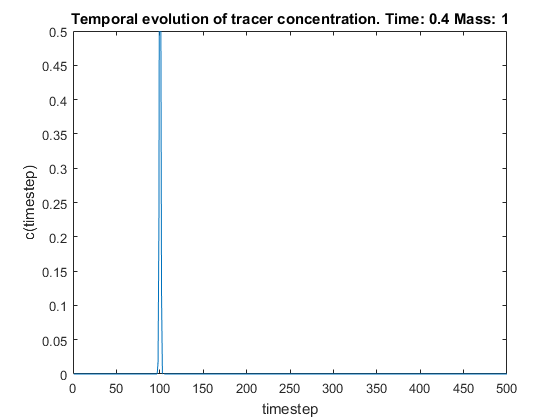
\includegraphics[width=\textwidth]{temporal1}
		{{\small Temporal evolution of the tracer at the beginning of simulation.}}    
	\end{subfigure}
	\begin{subfigure}[b]{0.8\textwidth}   
		\centering 
		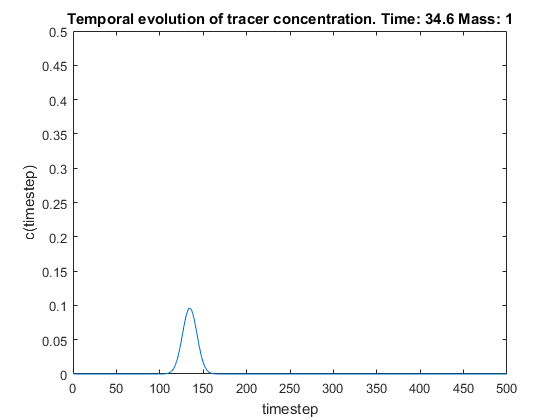
\includegraphics[width=\textwidth]{temporal2}
		{{\small Temporal evolution of the tracer further into simulation.}}    
	\end{subfigure}
\end{figure}

\begin{figure}[H]
	\centering
	\begin{subfigure}[b]{0.8\textwidth}   
		\centering 
		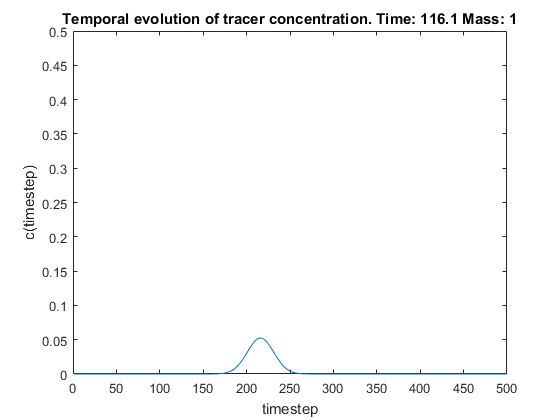
\includegraphics[width=\textwidth]{temporal3}
		{{\small Temporal evolution of the tracer after significant time.}}    
	\end{subfigure}
	\begin{subfigure}[b]{0.8\textwidth}   
		\centering 
		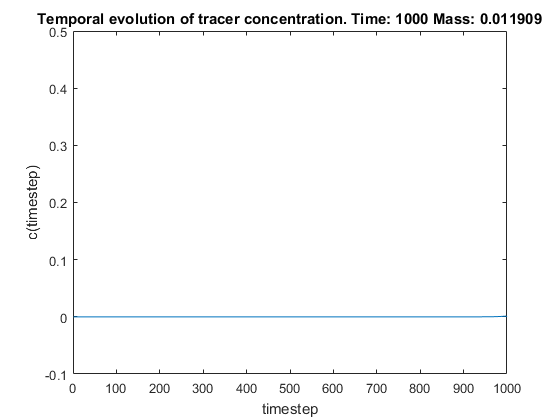
\includegraphics[width=\textwidth]{temporal4}
		{{\small Temporal evolution of the tracer at the end of simulation.}}    
	\end{subfigure}
\end{figure}

At the beginning of simulation the tracer concentration starts at its highest point and its curve becomes smaller and wider with time. At the very end the value is around 0. The explanation for this is that tracer has left the system. 

\begin{figure}[H]
	\centering
	\begin{subfigure}[b]{0.8\textwidth}   
		\centering 
		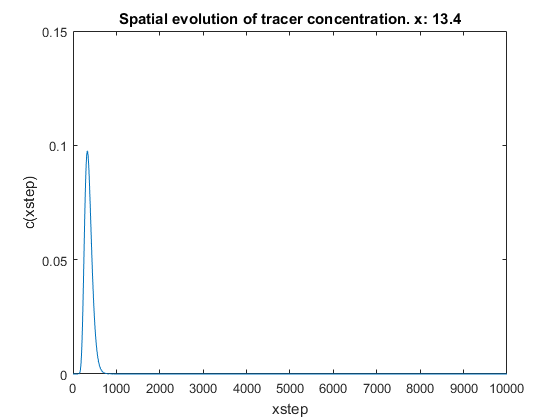
\includegraphics[width=\textwidth]{spatial1}
		{{\small Spatial evolution of the tracer at the beginning of simulation.}}    
	\end{subfigure}
	\begin{subfigure}[b]{0.8\textwidth}   
		\centering 
		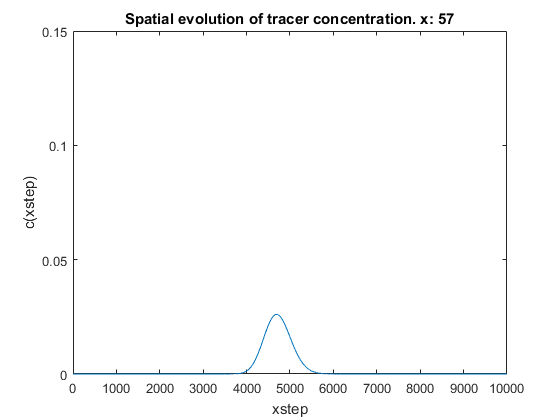
\includegraphics[width=\textwidth]{spatial2}
		{{\small Spatial evolution of the tracer further into simulation.}}    
	\end{subfigure}
\end{figure}

\begin{figure}[H]
	\centering
	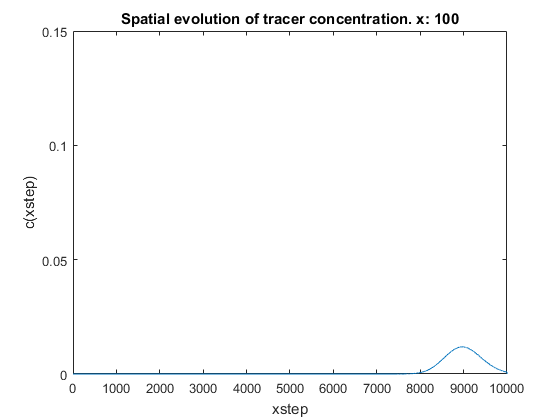
\includegraphics[width=\textwidth]{spatial3}
	{{\small Spatial evolution of the tracer at the end of simulation.}}    
\end{figure}

Results for spatial evolution are very similar to temporal one. The main difference is that the simulation is stopped when tracer reaches the end of the river.

\subsection{Numerical stability for different parameters}

When using numerical solution it is always necessary to make sure correct parameters were chosen. Otherwise it will lead to unexpected results. Numerical stability is property saying that for small changes of parameters there is small change in the outcome. When that's not the case the algorithm is considered \textit{unstable}.

Demonstrating what happens in this case can be as simple as looking at plots for various \textit{D} (dispersion coefficient), \textit{U} (advection coefficient), \textit{dt} and \textit{dx} parameters.

\begin{figure}[H]
	\centering
	\begin{subfigure}[b]{0.8\textwidth}   
		\centering 
		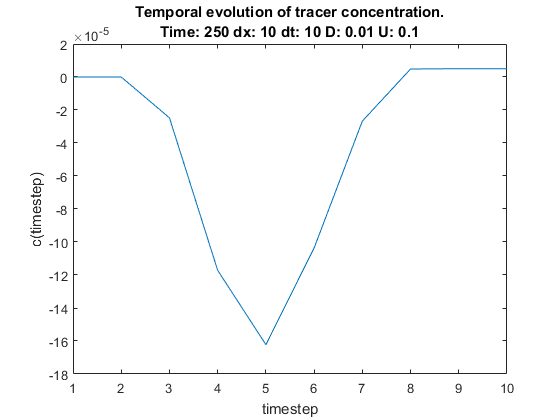
\includegraphics[width=\textwidth]{stability1}
		{{\small Testing numerical stability for different dx and dy parameters.}}    
	\end{subfigure}
	\begin{subfigure}[b]{0.8\textwidth}   
		\centering 
		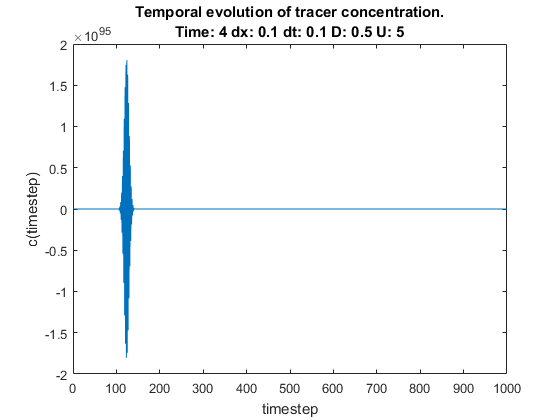
\includegraphics[width=\textwidth]{stability2}
		{{\small Testing numerical stability for different U and D parameters.}}    
	\end{subfigure}
\end{figure}


\subsection{Mass conservation law}
The law of conservation of mass states that for any system closed to all transfers of matter and energy, the quantity of mass is conserved over time.

It is possible to check if this law applies to the defined model by simply noticing that the total mass of the tracer present in the river is constant in time.

This can be confirmed looking at figures from section 2.2 where mass was included. It stops being constant only after long time when tracer has already left the system which is compliant to mass conservation law.

\section{Conclusion}

Over the course of this laboratory we implemented simple simulation of pollutants in the river using QUICKEST method which expressed differential equation as iteration formula.

Despite simplicity of the model we touched on the problem of numerical stability and checked the law of conservation of mass seeing differences in model behavior when the system is closed and open.

\end{document}
